% !TEX program = xelatex

% ==== Part1: 引入latex需要的package,支持不同的需求,如中文、图片 ====
\documentclass{article}
\usepackage[UTF8]{ctex} % 中文latex支持
\usepackage{graphicx} % 引入图片时需要的包
\usepackage{float}    % 插入图片的时候支持`H`这个位置选项
\usepackage{subcaption} % 插入多张图片到一个figure域中
\usepackage{hyperref}   % 插入超链接、TOC支持链接
\usepackage{amsmath,bm} % 一些数序符号、字符
\usepackage{listings}   % 插入代码块
% ==== 对引入的package配置 ====
\graphicspath{{images/}} % 配置graphicx这个包:指定图片存储的地方
\hypersetup{ % 设置超链接和url的显示样式
    colorlinks=true,
    linkcolor=blue,
    filecolor=magenta,      
    urlcolor=cyan,
    pdftitle={Overleaf Example},
    pdfpagemode=FullScreen,
    }
\urlstyle{same}

% ==== Part2: latex文档格式配置 ====
\newif\ifchinese % 定义一个条件变量: ifchinese, 作为控制条件编译的开关
\chinesetrue % 条件编译的控制开关,注释掉此部分内容,则对应部分不会被现实
\newif\ifchinese % 定义一个条件变量: ifchinese, 作为控制条件编译的开关
\chinesetrue % 条件编译的控制开关,注释掉此部分内容,则对应部分不会被现实

% ==== Part3: latex文档标题部分 ====
\title{基于RISC-V的嵌入式低功耗MCU设计}
\author{付杰}
\date{2023 年 4 月 19日 to \today}


% ==== Part4: latex文档正文部分 ====
\begin{document}
\maketitle
\newpage

\begin{abstract} % 摘要
  RISC-V指令集低功耗嵌入式实时响应MCU,五级流水线设计
  \par\textbf{关键字:} RISC-V, MCU, 低功耗
\end{abstract}
\newpage

\tableofcontents % 插入目录
\newpage


\section{MCU整体特点及实现方案}
\subsection{流水线}
\subsubsection{IF}
\begin{enumerate}
  \item \textbf{静态分支预测}:
  分支预测主要完成的任务是\textbf{方向预测和地址预测}\cite{riscv1}
    \begin{itemize}
      \item B-Type: FNBT
      \item JAL: 直接做静态预测,直接跳转
      \item \textbf{JALR}:只对x0, x1(JALR指令往往跟JAL指令成对出现,
        RISC-V中x1默认作为函数返回地址寄存器)做硬件加速;
        其余情况下不对JALR做分支预测
    \end{itemize}
  \item ITCM容量64kB\cite{riscv1}
  \item 压缩指令:需要处理压缩指令导致
    的\textbf{指令不对齐问题、PC更新问题}\cite{riscv1}
\end{enumerate}
\subsubsection{ID}
\begin{enumerate}
  \item 压缩指令译码方式有两种: 单独按照功能对压缩指令译码\cite{riscv1}、
    按照压缩指令跟32bits指令的对应关系,将其恢复成32bits指令再译码
\end{enumerate}
\subsubsection{EXE}
\begin{enumerate}
  \item 加法器: 进位链的生成是加法器设计的关键\cite{riscv1}
    \begin{enumerate}
      \item 超前进位加法器
      \item 行波进位加法器
      \item 并行前缀加法器
    \end{enumerate}
\end{enumerate}
\subsubsection{MEM}
\begin{enumerate}
  \item 访存指令的目标地址可以是非对齐的,但不强制要求 微架构硬件支持非对齐访存,而是可以通过异常处理程序完成该功能\cite{riscv1}
  \item RISC-V 架构明确规定了访存异常可以作为非精确异步异常处理。\\
    在变长两级、三级流水线中,LSU在第三级(第三级的指令看做已经commit),
    其后续的指令可能已经完成了,因此load/store指令不能精确异常\cite{riscv1}
\end{enumerate}
\subsubsection{WB}
\subsection{低功耗}
\begin{enumerate}
  \item \textbf{逻辑门控}\cite{riscv1}:加法器、移位器等运算资源内 部包含大量逻辑门,若在空闲时放任其翻转将造成大量功耗开销。\\
   使用逻辑门控的方法,在不使用运算资源时强制其输入为0,从而避免上述问题
 \item 多个电源域\cite{riscv1}:空闲时可将主域以及调试域的电源关闭而
    只保留常开域电源,以节省功耗
\end{enumerate}
\subsection{调试}
\begin{enumerate}
  \item 如果一款处理器不具备调试能力,那么一旦程序运行出现问题,开发 人员便束手无策。\\
    RISC-V 基金会并未发布标准的 RISC-V 调试架构文档,但是由 SiFive 开源推出的交互式调试方案获得了官方认证,具有较大影响力\cite{riscv1}
  \item 调试模式可以被视作一种特殊的中断处理,其与普通的异常处理不同在于:
    \begin{itemize}
      \item 断点 PC 保存至调试系统定义的 dpc 寄存器中而不是 epc 寄存器
      \item 中断相关信息需存入 dcsr 中而非 csr
      \item 进入中断处理后指令 PC 将跳转至 0x800(定义的调试程序的起始地址) 而非由 mtvec 所指定的 PC
      \item 处理器进入 Debug 模式,在此模式下处理器不再响应任何中断请求
      \item 调试中断的退出由 dret 指令控制而非 mret
    \end{itemize}
  \item 调试模块可以执行的功能:
    \begin{itemize}
      \item 读取 RISC-V 系统的状态
      \item 控制处理器的运行,包括暂停或按步运行等
      \item 向 RISC-V 系统的存储器写入数据
    \end{itemize}
  \item 实现调试需要的软硬件
    \begin{itemize}
      \item Host PC: gdb, gdbServer(OpenOCD)
      \item JTAG
      \item RISC-V Platform
        \begin{itemize}
          \item DTM(Dubug transform module):将JTAG信号转化成debug bus信号
          \item Debug Bus
          \item \textbf{DM(Debug Module)}:向RISC-V Core发送调试信号、控制调试、存储调试程序等
          \item RISC-V Core:支持调试
        \end{itemize}
    \end{itemize}
\end{enumerate}
\subsection{SoC}
\begin{figure}[H]
\begin{center}
  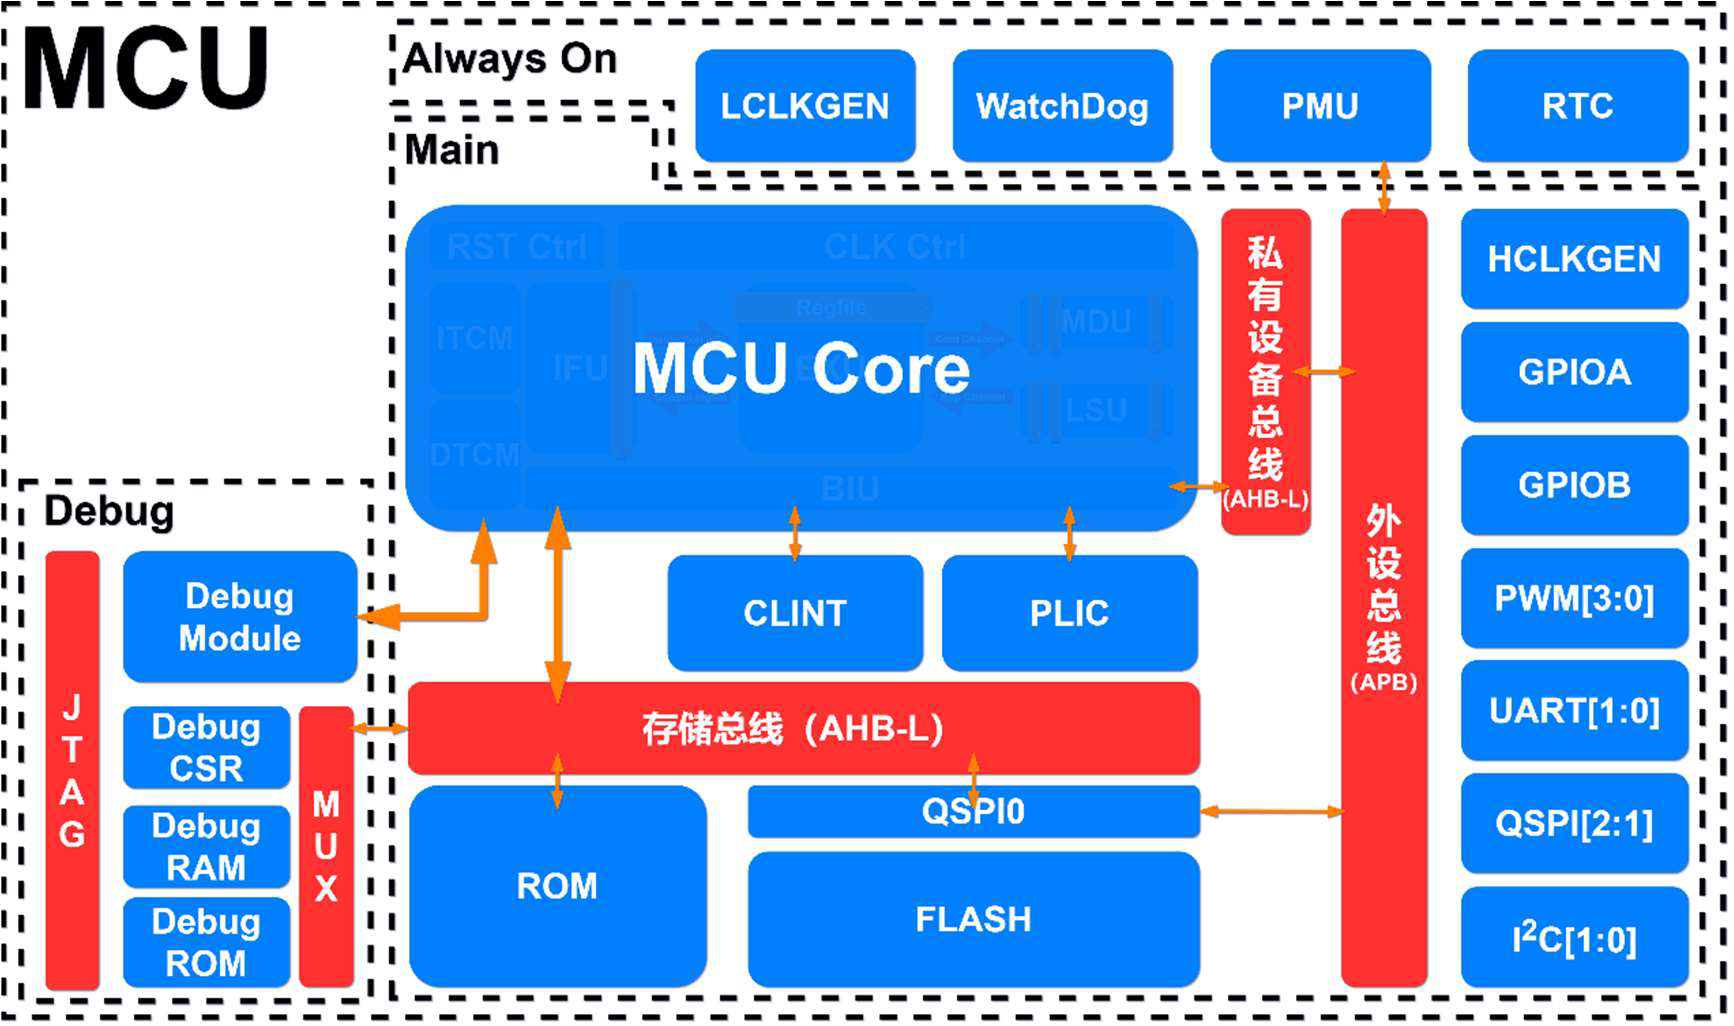
\includegraphics[width=\textwidth]{soc}
\end{center}
\caption{蜂鸟E203SoC}
\label{fig: SoC1}
\end{figure}

\subsection{加速器控制}
\subsection{MCU测试}
\subsubsection{SoC系统测试}
\begin{enumerate}
  \item RISC-V有自己的工具链和测试程序,可以通过Github下载\cite{riscv3}
  \item 高级语言编译成MCU上可以运行的程序,还需要提供板级支持包BSP(Board Support Package)\cite{riscv1},BSP提供如下支持:
    \begin{enumerate}
      \item MCU 硬件设备的地址分配信息
      \item 硬件设备的驱动函数
      \item 系统引导程序
      \item 中断、异常服务程序
      \item 系统链接脚本
      \item 高级语言运行库
    \end{enumerate}
\end{enumerate}
\subsubsection{处理器核测试}
简单的对\textbf{处理器核功能测试}可以通过Golden Model比较的方法测试\\ 
给软件模拟器,如\textbf{Spike}加载更处理器核同样的指令序列,然后比较每个周期的
处理器核的寄存器和内存的数据以及模拟器的寄存器和处理器核的信息\cite{riscv4}。 
如果二者的数据恒一致,则可以认为处理器核的功能是正确的

\section{Chisel}
\textbf{Chisel}将设计空间的抽象水平从\textbf{寄存器传输级} 的硬件层面提高到高层次的、\textbf{面向对象}的软件层面
\textbf{相对于Verilog的优点}: 支持高度参数化的电路生成器\cite{riscv2}
\begin{itemize}
  \item 代码更加高效:Chisel 的编译器框架可以实现电路的自动专业化和转换。 这意味着转变为 FPGA 优化版本的电路比未优化的版本运行得更快
  \item 自定义接口类型:Chisel 允许将基本的数据类型聚集成捆,以创建新的数据类型或方便捆绑信 号的使用
  \item 参数化:Chisel 允许参数化的函数、Chisel 也允许参数化的类
\end{itemize}
Chisel生成Verilog的三步流程:
\begin{enumerate}
  \item Chisel前端将Chisel代码生成FIR(Flexible Intermediate Representation)
  \item \textbf{优化}:为生成 RTL 提取优化 FIR 并读入自定义参数,得到FIRRTL
  \item 生成Verilog:后端根据优化的 FIRRTL 生成 Verilog
\end{enumerate}

Chisel \textbf{前后端示意图如下}:\cite{riscv3}
\begin{figure}[H]
\begin{center}
  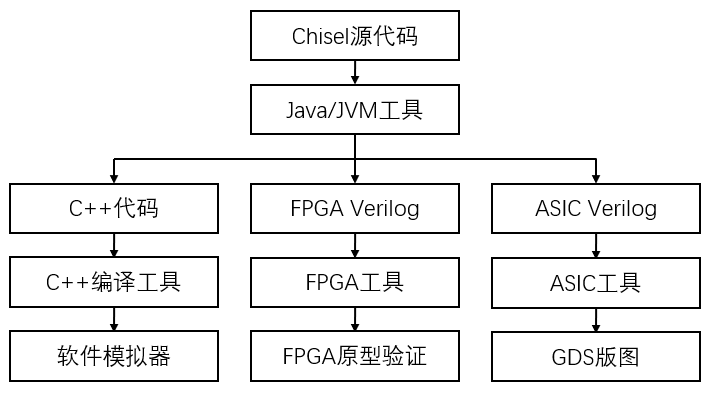
\includegraphics[width=\textwidth]{chisel}
\end{center}
\caption{基于 Chisel 源码的项目前后端流程示意图}
\label{fig: chisel}
\end{figure}




\newpage
\bibliography{mcuRef} % 参考文献源,存储所有的参考文献
\bibliographystyle{IEEEtran} % latex饮用参考文献时的格式

\end{document}

